% Included by main.tex; the preamble and references are shared.
\section{Spectral and planar preliminaries}\label{sec:preliminaries}

Let $\Omega\subset\mathbb R^2$ be a nonempty bounded connected open set with
$C^\infty$ boundary. Simple connectivity is not needed for the spectral comparison
below; it will be assumed explicitly in \cref{lem:conformal}.
All integrals over $\Omega$ are with respect to Lebesgue measure.
Write
\[
 \lambda_D=\inf_{0\ne v\in H_0^1(\Omega;\mathbb R)}
 \frac{\int_\Omega|\nabla v|^2}{\int_\Omega v^2},
 \qquad
 \lambda_N=\inf_{\substack{0\ne v\in H^1(\Omega;\mathbb R)\\
                          \int_\Omega v=0}}
 \frac{\int_\Omega|\nabla v|^2}{\int_\Omega v^2}.
\]
Here $\lambda_N$ denotes the first \emph{positive} Neumann eigenvalue, denoted
by $\mu$ in the source manuscript; the constant eigenfunctions have eigenvalue
zero. The Poincar\'e inequalities give $\lambda_D,\lambda_N>0$.
Compactness of the Sobolev embeddings into $L^2(\Omega)$ gives attainment of
these infima: normalize a minimizing sequence in $L^2$, take a weakly
convergent subsequence in the relevant Sobolev space and a strongly convergent
subsequence in $L^2$, and use weak lower semicontinuity of the gradient norm.

We record the variational facts used below. The spaces of complex-valued functions
are understood componentwise: $H^1(\Omega;\mathbb C)=H^1(\Omega;\mathbb R)
+iH^1(\Omega;\mathbb R)$, and similarly for $H_0^1$.

\begin{fact}[Neumann variational equality over $\mathbb C$]\label[fact]{fact:neumann-equality}
Define
\[
 a_N(f,g)=\int_\Omega\nabla f\cdot\overline{\nabla g}
          -\lambda_N\int_\Omega f\overline g.
\]
For $w\in H^1(\Omega;\mathbb C)$ with $\int_\Omega w=0$, one has
$a_N(w,w)\ge0$. Equality holds if and only if $w$ satisfies
\begin{equation}\label{eq:neumann-weak}
 \int_\Omega\nabla w\cdot\overline{\nabla\psi}
 =\lambda_N\int_\Omega w\overline\psi
 \qquad(\psi\in H^1(\Omega;\mathbb C)).
\end{equation}
\end{fact}
This is the standard Rayleigh variational characterization and its equality
case; see \cite[Theorem 11, pp.~6--7]{Gantumur}, with the Neumann form
domain $H^1(\Omega)$ and $k=2$ (the first eigenfunction is constant).
The complex version follows by separating real and imaginary parts.
\Cref{eq:neumann-weak} is the variational formulation of the
Laplacian eigenvalue problem with homogeneous Neumann boundary conditions:
the test space is all of $H^1(\Omega)$. On our smooth domain, elliptic
regularity \cite[Chapter III, Theorems 6.4 and 6.5]{Showalter} gives
$-\Delta w=\lambda_Nw$ in $\Omega$ and $\partial_\nu w=0$ on
$\partial\Omega$.

\begin{lemma}\label[lemma]{lem:spectral-gap}
One has $\lambda_N<\lambda_D$.
\end{lemma}
This is the first-mode case of Filonov's strict Dirichlet--Neumann
comparison \cite[Theorem, p.~414]{Fil05}. With eigenvalues counted from
one, including the constant Neumann eigenfunction, that theorem states
$\mu_{k+1}<\lambda_k$ for a domain of finite measure in dimension at
least two whenever $H^1(\Omega)\hookrightarrow L^2(\Omega)$ is compact.
Our bounded smooth planar domain satisfies these hypotheses. Since
$\Omega$ is connected, its zero Neumann eigenvalue is simple, so
$\lambda_N=\mu_2$ and $\lambda_D=\lambda_1$; taking $k=1$ gives the
asserted inequality.

Identify $\mathbb R^2$ with $\mathbb C$, and write
$\mathbb D=\{z\in\mathbb C:|z|<1\}$ and $S^1=\partial\mathbb D$.
Smoothness up to the boundary means smoothness in local coordinates on
the manifold with boundary $\overline\Omega$; in particular, all derivatives
extend continuously to the boundary. A boundary chart is a smooth local
diffeomorphism $F(s,t)$ that takes $t=0$ to $\partial\Omega$ and $t>0$
to $\Omega$, thereby flattening the boundary.

\begin{lemma}\label[lemma]{lem:conformal}
If $\Omega$ is simply connected, there is a conformal bijection
$\Phi:\mathbb D\to\Omega$ extending to a smooth diffeomorphism
$\overline{\mathbb D}\to\overline\Omega$. Its complex derivative
$\Phi'$ extends smoothly and is nonzero everywhere on
$\overline{\mathbb D}$.
\end{lemma}
\begin{proof}
The Riemann mapping theorem gives a conformal bijection
$\Phi:\mathbb D\to\Omega$, since $\Omega$ is nonempty, simply connected,
and a proper subdomain of $\mathbb C$.

The bounded simply connected domain $\Omega$ with smooth boundary is a
Jordan domain, meaning the bounded component of the complement of a
simple closed curve. Indeed, its compact smooth boundary is a finite disjoint
union of embedded circles; any additional boundary component would
bound a hole, around which an interior loop has nonzero winding number
and cannot contract in $\Omega$. Thus there is only the outer boundary
curve, and $\Omega$ is its bounded complementary component.

Carath\'eodory's boundary extension theorem gives a homeomorphic extension
$\Phi:\overline{\mathbb D}\to\overline\Omega$.
For a Jordan domain with $C^{k,\alpha}$ boundary, where $k\ge1$ and
$0<\alpha<1$, the Kellogg--Warschawski theorem makes this extension
$C^{k,\alpha}$ and gives a continuous nonvanishing extension of $\Phi'$;
see \cite[Chapter 2 and Theorems 3.5 and 3.6]{Pom92}.
Here $C^{k,\alpha}$ means that regular local boundary parametrizations
have $k$ derivatives, with the $k$th H\"older continuous of exponent
$\alpha$. Fixing $\alpha\in(0,1)$, our $C^\infty$ boundary satisfies
this hypothesis for every $k$. Thus $\Phi$ and $\Phi'$ extend smoothly,
with $\Phi'\ne0$ everywhere on $\overline{\mathbb D}$.
To check that the inverse is also smooth at the boundary, extend $\Phi$
locally as a smooth real map across $S^1$. The Cauchy--Riemann equations
extend to $S^1$ by continuity, giving
\[
 \det D\Phi=|\Phi'|^2>0.
\]
The real inverse function theorem therefore gives local smooth inverses.
Their restrictions agree with the global inverse supplied by the
homeomorphism, so that inverse is smooth on $\overline\Omega$.
This proves the asserted diffeomorphism of closures.
\end{proof}

For the remainder of this section assume that $\Omega$ is simply connected,
and fix the map $\Phi$ from \cref{lem:conformal}. Write $ds$ for
arclength on $S^1$, of total mass $2\pi$, and $d\sigma$ for arclength
on $\partial\Omega$. Let $V$ be the real Neumann eigenspace for
$\lambda_N$; its members satisfy the variational formulation
\begin{equation}\label{eq:V-weak}
 \int_\Omega\nabla v\cdot\nabla\psi
 =\lambda_N\int_\Omega v\psi
 \qquad(\psi\in H^1(\Omega;\mathbb R)).
\end{equation}
The full $H^1$ test space encodes the homogeneous Neumann boundary
condition; compactly supported tests alone would encode only the interior
Laplacian equation. They are smooth up to the boundary and satisfy
$-\Delta v=\lambda_Nv$ in $\Omega$ and $\partial_\nu v=0$ on
$\partial\Omega$. Taking $\psi=1$ gives $\int_\Omega v=0$, since
$\lambda_N>0$.

\begin{lemma}\label[lemma]{lem:boundary-weight}
There is a fixed $\beta\in C^\infty(S^1)$, strictly positive everywhere,
such that every $v\in V$ has boundary trace
$h_v=(v\circ\Phi)|_{S^1}$ satisfying
\[
 \int_{S^1}\beta h_v\,ds=0.
\]
If $v\ne0$, then $h_v$ is not identically zero and takes both positive
and negative values.
\end{lemma}
\begin{proof}
Consider the symmetric bilinear form
\[
 b(f,g)=\int_\Omega\nabla f\cdot\nabla g
        -\lambda_N\int_\Omega fg
 \qquad(f,g\in H_0^1(\Omega;\mathbb R)).
\]
The definition of $\lambda_D$ gives the Dirichlet inequality
\begin{equation}\label{eq:dirichlet-inequality}
 \int_\Omega|\nabla f|^2\ge\lambda_D\int_\Omega f^2
 \qquad(f\in H_0^1(\Omega;\mathbb R)).
\end{equation}
By \cref{lem:spectral-gap}, $\lambda_N<\lambda_D$, so
\[
 b(f,f)\ge
 \left(1-\frac{\lambda_N}{\lambda_D}\right)
 \int_\Omega|\nabla f|^2
 \ge c\|f\|_{H^1(\Omega)}^2
\]
for some $c>0$, using the Poincar\'e inequality in the last step.
Thus $b$ is coercive. It is also continuous, and
$\eta\mapsto\int_\Omega\eta$ is a continuous linear functional on
$H_0^1(\Omega)$. The Riesz representation theorem applied to the inner
product $b$, or equivalently Lax--Milgram, gives a unique real
$L\in H_0^1(\Omega)$ such that
\begin{equation}\label{eq:L-weak}
 b(L,\eta)=\int_\Omega\eta
 \qquad(\eta\in H_0^1(\Omega;\mathbb R)).
\end{equation}
This is the weak Dirichlet problem
\[
 (-\Delta-\lambda_N)L=1\quad\text{in }\Omega,
 \qquad \operatorname{Tr}L=0.
\]
Here $\operatorname{Tr}:H^1(\Omega)\to L^2(\partial\Omega)$ is the
bounded extension of boundary restriction for smooth functions;
$H_0^1(\Omega)$ is precisely its kernel.
For this coercive solvability argument with a negative zeroth-order
coefficient, see \cite[Example 4.14, p.~100]{Hunter}; the displayed
estimate verifies its hypothesis using the optimal Dirichlet constant.
To justify smoothness, rewrite the equation as
$-\Delta L=1+\lambda_NL$. Initially its right-hand side is in $L^2$,
so boundary regularity gives $L\in H^2(\Omega)$. Repeated application
of higher-order boundary regularity gives $L\in H^k(\Omega)$ for every
integer $k$, and Sobolev embedding then gives
$L\in C^\infty(\overline\Omega)$; see
\cite[Theorem 4.31 and Corollary 4.32, p.~116]{Hunter}.

Define $L^-=\max\{-L,0\}=(|L|-L)/2$. Absolute values preserve
$H^1(\Omega)$ and commute with the trace, so $|L|\in H_0^1(\Omega)$
because $L\in H_0^1(\Omega)$. Thus $L^-\in H_0^1(\Omega)$.
The Sobolev chain rule gives
$\nabla L^-=-\mathbf1_{\{L<0\}}\nabla L$ almost everywhere.
Almost everywhere on $\{L<0\}$,
$L=-L^-$ and $\nabla L=-\nabla L^-$; on its complement $L^-$ and
$\nabla L^-$ vanish almost everywhere. Taking $\eta=L^-$ in
\cref{eq:L-weak} therefore gives
\[
 -b(L^-,L^-)=b(L,L^-)=\int_\Omega L^-\ge0.
\]
Coercivity forces $L^-=0$, and thus $L\ge0$ everywhere by continuity.
Consequently
\[
 -\Delta L=1+\lambda_NL>0\quad\text{in }\Omega.
\]
In fact $L>0$ in $\Omega$: an interior zero would be a local minimum
of the smooth nonnegative function $L$, where $\Delta L\ge0$, contrary
to the displayed equation. Put $u=-L$. Then $u$ is smooth up to the
boundary, $u<0$ in $\Omega$, $u=0$ on $\partial\Omega$, and
$\Delta u=1+\lambda_NL>0$. At each $p\in\partial\Omega$, smoothness
of the boundary gives the interior sphere condition: there is a ball
$B_r(b)\subset\Omega$ tangent to $\partial\Omega$ at $p$.
The Hopf boundary point lemma states that if a function is $C^2$ in
the domain and $C^1$ up to the boundary, satisfies $\Delta u\ge0$ and
$u<M$ in the domain, and has $u(p)=M$ at a boundary point satisfying
the interior sphere condition, then $\partial_\nu u(p)>0$.
Applied here with $M=0$,
it gives $\partial_\nu u(p)>0$; see
\cite[Lemma 2.21, p.~29]{Hunter}. Consequently,
\begin{equation}\label{eq:L-normal}
 -\partial_\nu L>0\quad\text{on }\partial\Omega,
\end{equation}
where $\nu$ is the outward unit normal.

For $v\in V$, the equations $-\Delta v=\lambda_Nv$ and
$(-\Delta-\lambda_N)L=1$, followed by Green's identity, give
\[
 \begin{aligned}
 0=\int_\Omega v
 &=\int_\Omega\bigl(v(-\Delta L)-L(-\Delta v)\bigr)\\
 &=\int_{\partial\Omega}
       \bigl(L\partial_\nu v-v\partial_\nu L\bigr)\,d\sigma\\
 &=-\int_{\partial\Omega}v\partial_\nu L\,d\sigma.
 \end{aligned}
\]
All functions are smooth up to the boundary, so this is the classical
Green identity. In the last line we used $L=0$ and
$\partial_\nu v=0$ on $\partial\Omega$.
The boundary diffeomorphism $\Phi:S^1\to\partial\Omega$ changes
arclength by $d\sigma=|\Phi'(s)|\,ds$. Hence
\[
 0=\int_{S^1}\beta(s)h_v(s)\,ds,
 \qquad
 \beta(s)=|\Phi'(s)|\,(-\partial_\nu L)(\Phi(s)).
\]
This $\beta$ depends only on $\Omega$ and the fixed parametrization
$\Phi$, and is smooth and strictly positive by
\cref{eq:L-normal} and \cref{lem:conformal}.

If $h_v$ were identically zero, boundary surjectivity of $\Phi$ would
give $\operatorname{Tr}v=0$, hence $v\in H_0^1(\Omega)$.
Testing \cref{eq:V-weak} with $\psi=v$ and applying
\cref{eq:dirichlet-inequality} would give
\[
 \lambda_D\int_\Omega v^2
 \le\int_\Omega|\nabla v|^2
 =\lambda_N\int_\Omega v^2.
\]
The strict spectral gap forces $v=0$. Thus $v\ne0$ implies that $h_v$
is a nonzero continuous function. If it were everywhere nonnegative,
strict positivity of $\beta$ and continuity would give
$\int_{S^1}\beta h_v\,ds>0$; if it were everywhere nonpositive, the
integral would be negative. Both contradict its zero weighted integral.
Therefore $h_v$ takes both signs.
\end{proof}

\begin{fact}[Separation by a disk crosscut]\label[fact]{fact:crosscut}
A crosscut of $\mathbb D$ is a simple arc $\alpha$, the image of a
continuous injective map $[0,1]\to\overline{\mathbb D}$, whose distinct
endpoints $s_1,s_3$ lie on $S^1$ and whose remaining points lie in
$\mathbb D$. If $I_1,I_2$ are the two closed circle arcs between those
endpoints, then $\mathbb D\setminus\alpha$ has exactly two connected
components $C_1,C_2$, numbered so that
\[
 \partial C_j=\alpha\cup I_j\qquad(j=1,2).
\]
Consequently, if $s_1,s_2,s_3,s_4$ are cyclically ordered on $S^1$,
every continuous path from $s_2$ to $s_4$ whose remaining points lie
in $\mathbb D$ intersects $\alpha$ inside $\mathbb D$.
\end{fact}
The separation statement is the crosscut form of the Jordan curve
theorem; see \cite[Section 14.2, ``Crosscuts'']{Conway}.
To justify the consequence explicitly, number the circle arcs so that
$s_2\in I_1\setminus\{s_1,s_3\}$ and
$s_4\in I_2\setminus\{s_1,s_3\}$. Then $s_2\notin\overline{C_2}$
and $s_4\notin\overline{C_1}$. If the path avoided $\alpha$, its
interior points near $s_2$ would belong to $C_1$ and those near $s_4$
to $C_2$. Its connected interior image cannot meet both components
while remaining in $\mathbb D\setminus\alpha$.

\begin{lemma}\label[lemma]{lem:nodal-components}
For every $0\ne v\in V$, the sets $\{v>0\}$ and $\{v<0\}$ in
$\Omega$ are connected. The boundary trace $h_v$ cannot have four
cyclically ordered points with strictly alternating signs.
\end{lemma}
\begin{proof}
Both sign sets are nonempty: $v$ is continuous, nonzero and has mean
zero. For any component $U$ of either sign set, define
$v_U=v\mathbf1_U$. The standard nodal-domain restriction result gives
$v_U\in H^1(\Omega)$; see \cite[Lemma 3.6, equation (3.1)]{Kluitenberg},
specialized to the Euclidean Laplacian with Neumann boundary conditions.
Its weak gradient satisfies
\begin{equation}\label{eq:restriction-gradient}
 \nabla v_U=\mathbf1_U\nabla v\quad\text{almost everywhere in }\Omega.
\end{equation}
Indeed, the gradients agree on $U$, and the weak gradient of a real
$H^1$ function vanishes almost everywhere on its zero set. Applied to
$v_U$, this gives $\nabla v_U=0$ almost everywhere on $\{v_U=0\}$.
We may therefore take $\psi=v_U$ in \cref{eq:V-weak}, obtaining
\begin{equation}\label{eq:component-energy}
 \int_\Omega|\nabla v_U|^2
 =\lambda_N\int_\Omega v_U^2.
\end{equation}
Suppose there were at least three distinct sign components
$U_1,U_2,U_3$. Set $A_j=\int_\Omega v_{U_j}$ for $j=1,2$.
Each $A_j$ is nonzero, because $v_{U_j}$ has one strict sign on the
nonempty open component $U_j$ and is zero elsewhere. The function
\[
 f=A_2v_{U_1}-A_1v_{U_2}
\]
belongs to $H^1(\Omega)$, has mean zero, and is nonzero, for example
on $U_1$. The two restrictions and their gradients vanish almost
everywhere outside the respective disjoint sets $U_1,U_2$, by
\cref{eq:restriction-gradient}; hence all cross terms in their energies
are zero.
Thus \cref{eq:component-energy} gives
\[
 \int_\Omega|\nabla f|^2=\lambda_N\int_\Omega f^2.
\]
By \cref{fact:neumann-equality}, $f$ is a weak Neumann eigenfunction.
Elliptic regularity makes it smooth in the interior, where
$-\Delta f=\lambda_N f$. Since $f$ vanishes on the nonempty open set
$U_3$, unique continuation for this elliptic equation forces $f=0$
throughout the connected domain $\Omega$; see
\cite[Theorem, pp.~235--236]{Aronszajn}. Here the principal coefficients
are constant and the zeroth-order coefficient is bounded, so the
theorem applies. This is a contradiction. There are therefore
exactly two sign components, one positive and one negative.

For the boundary assertion, put $\widehat v=v\circ\Phi$ on
$\overline{\mathbb D}$. The homeomorphism $\Phi$ makes the interior
sets $P=\{\widehat v>0\}\cap\mathbb D$ and
$N=\{\widehat v<0\}\cap\mathbb D$ connected and open.
Suppose $s_1,s_2,s_3,s_4\in S^1$ are distinct and cyclically ordered,
with positive values at $s_1,s_3$ and negative values at $s_2,s_4$;
the other alternating pattern is handled by replacing $v$ by $-v$.
Continuity gives short inward radial segments at $s_1$ and $s_3$
whose values are strictly positive, including their boundary endpoints.
Their interior endpoints can be joined by a finite polygonal path in
$P$. Indeed, an open connected subset of $\mathbb R^2$ is polygonally
connected: the points reachable from a fixed point by finite polygonal
paths form a relatively open set with relatively open complement.
The union of this path and the two radial segments contains a simple
polygonal arc $\alpha$ from $s_1$ to $s_3$. To obtain this arc,
subdivide the finitely many segments
at their intersections and at endpoints of overlaps. The resulting
finite connected embedded graph has a simple graph path between
$s_1$ and $s_3$. Its image is the required arc, whose other points
lie in $P$.

Construct in the same way a continuous path $\gamma$ from $s_2$ to
$s_4$, with every other point in $N$, using negative radial segments
and a polygonal path in $N$. By \cref{fact:crosscut}, $\gamma$ meets
$\alpha$ inside $\mathbb D$. At the intersection $\widehat v$ would
be both strictly positive and strictly negative. This contradiction
proves the boundary assertion. \Cref{fig:alternating-signs} illustrates
the configuration; the separation argument does not impose any
straightness or curvature condition on the connecting paths.
\end{proof}

\begin{figure}[htbp]
\centering
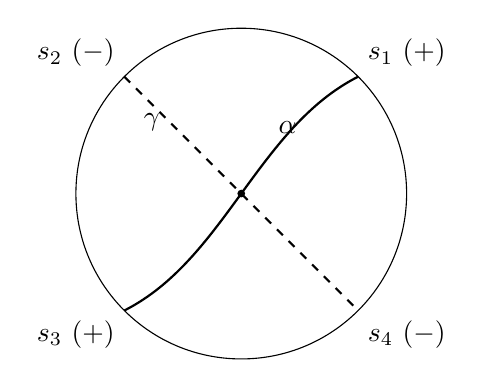
\begin{tikzpicture}[scale=1.4]
 \draw (0,0) circle (1.5);
 \draw[thick] (45:1.5) .. controls (0.15,0.6) and (-0.15,-0.6) .. (225:1.5);
 \draw[dashed,thick] (135:1.5) -- (315:1.5);
 \fill (0,0) circle (0.035);
 \node[above right] at (45:1.5) {$s_1\ (+)$};
 \node[above left] at (135:1.5) {$s_2\ (-)$};
 \node[below left] at (225:1.5) {$s_3\ (+)$};
 \node[below right] at (315:1.5) {$s_4\ (-)$};
 \node[right] at (0.25,0.6) {$\alpha$};
 \node[left] at (-0.65,0.65) {$\gamma$};
\end{tikzpicture}
\caption{Schematic of the forbidden alternating-sign configuration.
The positive crosscut $\alpha$ joins $s_1$ to $s_3$. The putative
negative path $\gamma$ joins the other two boundary points and must
intersect $\alpha$ by \cref{fact:crosscut}. The particular shapes drawn
are illustrative; the theorem applies to the paths constructed in
\cref{lem:nodal-components}.}\label{fig:alternating-signs}
\end{figure}

The following bound is due to Nadirashvili
\cite[Theorem 3, p.~227]{Nadirashvili}; see also
\cite[Proposition 2.5]{BanuelosBurdzy}. We give the boundary-sign proof.

\begin{proposition}\label[proposition]{prop:multiplicity}
The real eigenspace $V$ has dimension at most two.
\end{proposition}
\begin{proof}
Suppose $\dim_{\mathbb R}V\ge3$. Consider the real linear map
\[
 T:V\to\mathbb R^2,\qquad
 T(v)=\left(\int_{S^1}\beta h_v\cos\theta\,ds,
             \int_{S^1}\beta h_v\sin\theta\,ds\right),
 \qquad s=e^{i\theta}.
\]
Its rank is at most two, so its kernel contains a nonzero $v$.
By \cref{lem:boundary-weight}, the trace $h=h_v$ is nonzero, takes
both signs, and satisfies
\begin{equation}\label{eq:three-moments}
 \int_{S^1}\beta h\,ds
 =\int_{S^1}\beta h\cos\theta\,ds
 =\int_{S^1}\beta h\sin\theta\,ds=0.
\end{equation}

Choose a strictly negative point $e^{i\theta_0}$ and cut the circle
there, parametrizing the other points by
$\theta\in(\theta_0,\theta_0+2\pi)$. Write
$H(\theta)=h(e^{i\theta})$, $B(\theta)=\beta(e^{i\theta})$, and
\[
 A=\{\theta\in(\theta_0,\theta_0+2\pi):H(\theta)>0\},
 \qquad a=\inf A,\quad b=\sup A.
\]
The set $A$ is nonempty and open. Continuity and strict negativity at
the cut give negative neighbourhoods at both ends of the angle
interval. Therefore
\[
 \theta_0<a<b<\theta_0+2\pi.
\]
Continuity gives $H(a)=H(b)=0$, and the definitions give $H\le0$
outside $[a,b]$. There is no negative value at any
$\theta\in(a,b)$: the definitions of infimum and supremum provide
positive angles $\theta_-<\theta<\theta_+$ in $A$. The cut point,
$e^{i\theta_-}$, $e^{i\theta}$ and $e^{i\theta_+}$ would then have
strictly alternating signs in cyclic order, contradicting
\cref{lem:nodal-components}. Hence $H\ge0$ on $[a,b]$.

Set $c=(a+b)/2$ and $d=(b-a)/2\in(0,\pi)$, and define the
$2\pi$-periodic function
\[
 F(\theta)=\cos(\theta-c)-\cos d.
\]
On the circle, $F>0$ precisely on the arc represented by $(a,b)$,
$F=0$ at its endpoints, and $F<0$ on the complementary open arc.
This follows from strict decrease of cosine on $[0,\pi]$, using
angular distance from $c$ in $[0,\pi]$. Thus $FH\ge0$ everywhere,
and $FH>0$ on the nonempty open set $A$. Since $B>0$,
\[
 \int_{\theta_0}^{\theta_0+2\pi} B(\theta)F(\theta)H(\theta)\,d\theta>0.
\]
On the other hand,
\[
 F(\theta)=\cos c\cos\theta+\sin c\sin\theta-\cos d,
\]
so \cref{eq:three-moments}, together with $ds=d\theta$, makes this
same integral zero. The contradiction proves $\dim_{\mathbb R}V\le2$.
\end{proof}
